\chapter{Results}

\label{cha:results}

\ifdraft{In this section you discuss any issues that came up while developing
    the system.  If you found something particularly interesting,
    difficult, or an important learning experience, put it here.  This is
    also a good place to put additional figures and data.}

In this section we discuss the results of considering HLC within the game Breakthrough, using a Concept Activation vector for evaluating how the neural network recognizes the HLC's. We first evaluate the neural network against various agents to validate that it has learned how to play the game. Secondly, we take a look at the changes in the emphasis of the neural network during training. The main point of interest there being whether the neural network notices simple HLCs early then stops considering them as the network improves.

\section{Evolution of the neural networks win rate}

\begin{figure}
    \begin{small}
        \begin{center}
            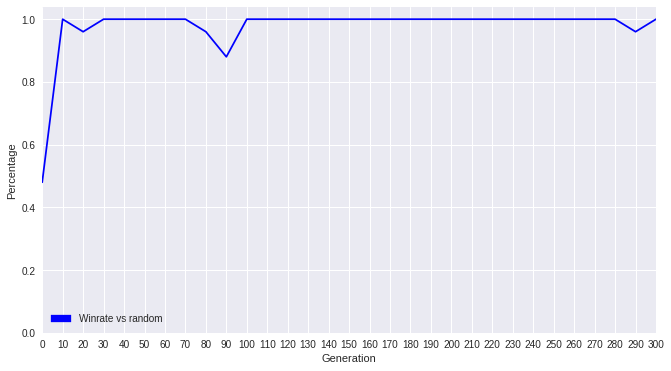
\includegraphics[width=0.7\textwidth]{graphics/winratevsrandom.png}
        \end{center}
        \caption{Winrate vs random agent}
        \label{fig:winratevsrandom}
    \end{small}
\end{figure}

\begin{figure}
    \begin{small}
        \begin{center}
            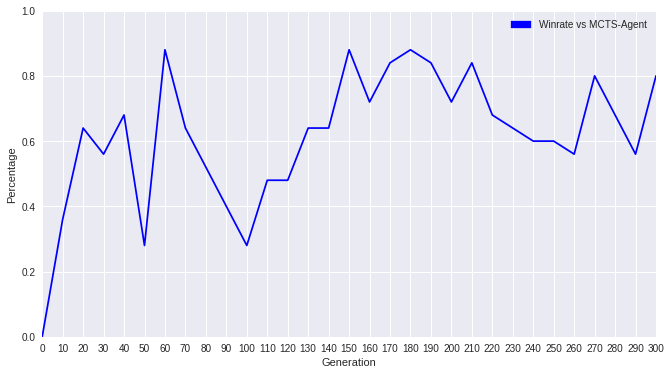
\includegraphics[width=0.7\textwidth]{graphics/winratevsmcts.png}
        \end{center}
        \caption{Winrate vs monte carlo tree search agent}
        \label{fig:winratevsmcts}
    \end{small}
\end{figure}

\begin{figure}
    \begin{small}
        \begin{center}
            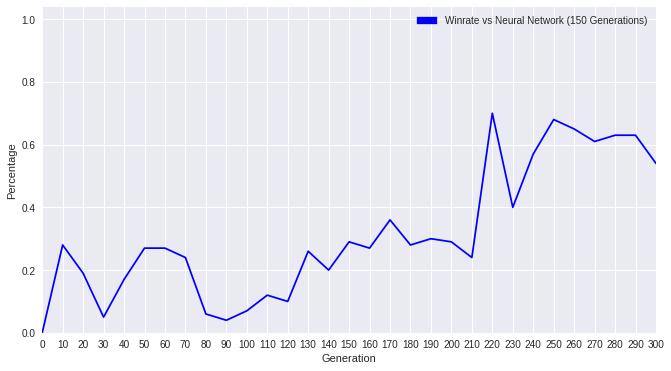
\includegraphics[width=0.7\textwidth]{graphics/winratevsneuralnetwork.png}
        \end{center}
        \caption{Winrate vs neural network trained for 150 generations}
        \label{fig:winratevsneuralnetwork}
    \end{small}
\end{figure}

Examining the neural network is only interesting if the neural network can effectively play the game. We first examine the history neural network playing against an agent that only takes random moves, on every $10$ generations. The win rate over generations can be seen in Figure \ref{fig:winratevsrandom}. It is clear that very early on in the training process, almost immediately after generation $10$ our agent performs nearly perfectly against the random agent. This implies that the agent does indeed learn some strategy in the game. The next agent we tried the neural network against, was an agent that does regular Monte-Carlo tree search on the game space with $100$ iterations of rollout for each move. A graph showing the win rate over generations can be seen in Figure \ref{fig:winratevsmcts}. Again, quickly our agent learns some strategy and can win often, but doesn't achieve a perfect win rate after $300$ generations. The last agent we tested against was the neural network itself, although only trained to $150$ generations. A graph showing the win rate can be seen in Figure \ref{fig:winratevsneuralnetwork}. As expected the agent performs poorly until it has trained for more than $150$ generations.

These results imply that our agent certainly understands how to play the game of breakthrough to a certain level. However, it should be stated that as we the creators attempt to compete against the agent it generally loses in a way that we would hope the agent should be able to play against. It is likely that as we train the neural network more it will become better.

\section{Evaluating the improvements of the neural network over generations}

To test which HLC the neural network places its emphasis on during training we trained a neural network for $300$ generations, taking snapshots of the network every $10$ generations. Then we had the neural network play against itself for $100$ games collecting the states it encountered during play. These states were then examined by a concept activation vector representing these HLCs.

We test four concepts \textit{Numbers Advantage}, \textit{Aggressiveness}, \textit{Unity}, and \textit{Lorentz-Horey}.

\subsection{Description of concepts}

\begin{figure}
    \begin{small}
        \begin{center}
            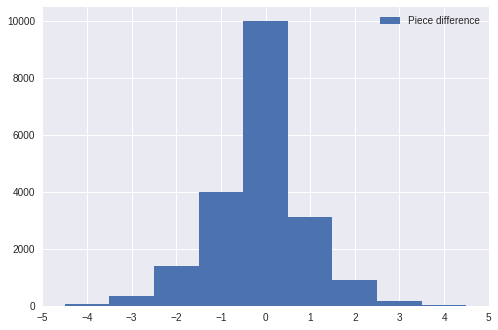
\includegraphics[width=0.95\textwidth]{graphics/dist_number_adv}
        \end{center}
    \end{small}
    \caption{Distribution of piece amount difference}
    \label{fig:dist_number_adv}
\end{figure}

The first concept we examine is Numbers Advantage which conveys the idea of having more pawns than your opponent. When faced with a board it is difficult to argue for whether having a single pawn up on your opponent constitues as Numbers Advantage or three. In order to an appropriate value for this case we used the neural network that had been trained for $300$ generations to generate $20000$ unique states. The distribution of the difference of pawns for each player can be seen in Figure~\ref{fig:dist_numbers_adv}. From examining the distribution and examining samples we selected the breakpoint of $2$, meaning that if you have $2$ pieces on your opponent you are in a state that has this concept. From the $20000$ states only $5.5\%$ of states have this property.

\begin{figure}
    \begin{small}
        \begin{center}
            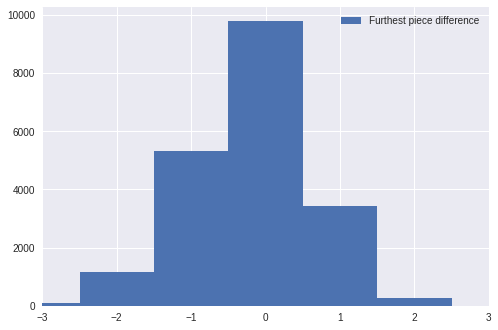
\includegraphics[width=0.95\textwidth]{graphics/dist_aggressiveness}
        \end{center}
        \caption{Distribution of difference of furthest pawns}
        \label{fig:dist_aggressiveness}
    \end{small}
\end{figure}


The next concept is Aggressiveness, which describes how much closer your furthest piece is to the opponents edge than your opponents furthest piece to your edge. This is then the minimum amount of how many moves it will take you to win the game. A distribution of these values can be seen in Figure~\ref{fig:dist_aggressiveness}. We examined the distribution, and sampled states from various breaking points and decided on the value of $\geq 1$. That is if the value of a state's furthest piece difference is greater than or equal to $1$ that state has the concept of aggressiveness.

\begin{figure}
    \begin{small}
        \begin{center}
            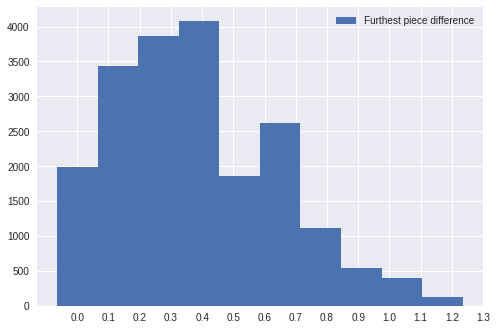
\includegraphics[width=0.95\textwidth]{graphics/dist_unity}
        \end{center}
        \caption{Difference of distance from center}
        \label{fig:dist_unity}
    \end{small}
\end{figure}








\subsection{Numbers Advantage}

Firstly there is the numbers advantage HLC, where the number of pawns the player has minus the number of pawns the opponent had, the breakpoint we selected was $2$ meaning that if you have $2$ more pawns then your opponent, you're in a position where a HLC called numbers advantage is present.

\begin{figure}[]
    \centering
    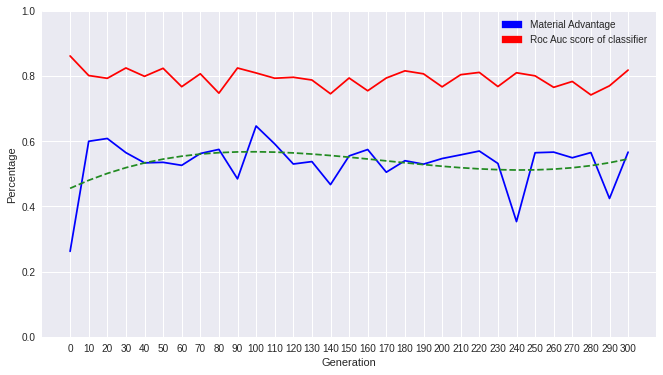
\includegraphics[width=0.7\textwidth]{graphics/number_pawns_trend}
    \caption{Percentage of selected states containing the HLC numbers advantage}
    \label{fig:numberadvantage}
\end{figure}

The Figure \ref{fig:numberadvantage}. shows that throughout training the numbers advantage HLC is only ever a slight factor in the selection of states and we can say that the neural network doesn't consider number advantage in its selection process.

The second HLC we examined was aggressiveness, which is a state in which your most advanced pawn is $2$ or more squares further than the opponents most advanced pawn.

\begin{figure}[]
    \centering
    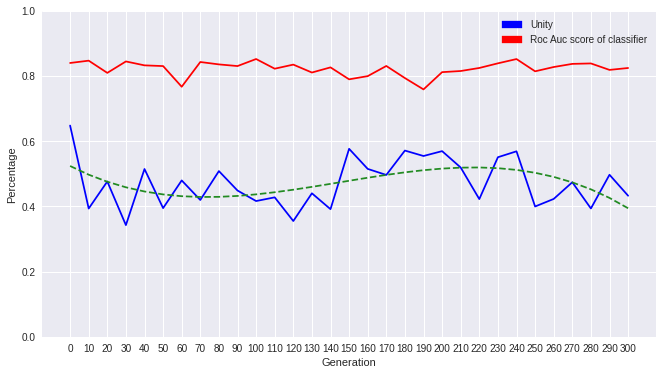
\includegraphics[width=0.7\textwidth]{graphics/most_advanced_trend.png}
    \caption{Percentage of selected states containing the HLC aggressiveness}
    \label{fig:aggressiveness}
\end{figure}

From Figure \ref{fig:aggressiveness}. we can see that the aggressiveness HLC is a growing factor over as the neural network is trained. Generally, when your opponent is not skilled this strategy is considered a good one.

The third HLC that we examined was unity, the unity HLC represents the absolute average distance of your pawns from the center row of your pawns. This HLC is calculated as the row of your furthest pawn from the starting row $r_{far}$, the row of your nearest pawn from the starting row $r_{near}$. Finding the middle row is then $\frac{r_{far} + r_{near}}{2}$, we then take the absolute of the average distance from the pawns to that row. To find the point at which this value relates to a state with the HLC unity, we sampled a myriad of states and decided on the value of $0.35$. The value of $0.35$ generally allows your states to have two rows that have the majority of the pawns and one or two pawns one row away from the group.

\begin{figure}[]
    \centering
    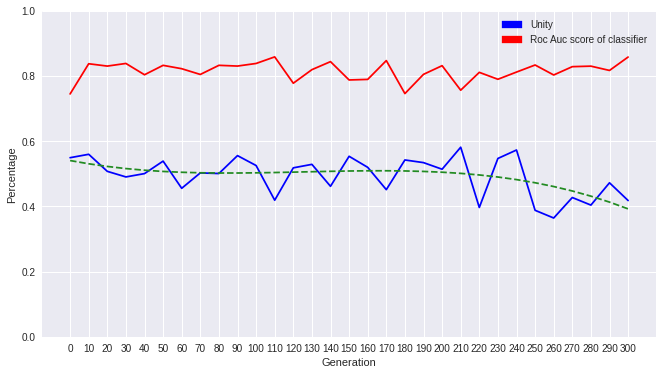
\includegraphics[width=0.7\textwidth]{graphics/unity_trend.png}
    \caption{Percentage of selected states containing the HLC unity}
    \label{fig:unity}
\end{figure}

The literature of breakthrough implies that being patient and waiting until your opponent makes a mistake is generally the preferred strategy for winning. the concept activation vector for Unity is not often triggered and is relatively stable at $50\%$ througout training.

\begin{table}[]
    \centering
    \begin{tabular}{|c|c|c|c|c|c|}
        \hline
        5  & 15 & 5  & 5  & 15 & 5  \\\hline
        2  & 3  & 3  & 3  & 3  & 2  \\\hline
        4  & 6  & 6  & 6  & 6  & 4  \\\hline
        7  & 10 & 10 & 10 & 10 & 7  \\\hline
        11 & 15 & 15 & 15 & 15 & 11 \\\hline
        21 & 21 & 21 & 21 & 21 & 21 \\\hline
    \end{tabular}
    \caption{Lorentz-Horey cell values, from white players point of view}
    \label{table:lorentzcell}
\end{table}

\begin{figure}
    \begin{small}
        \begin{center}
            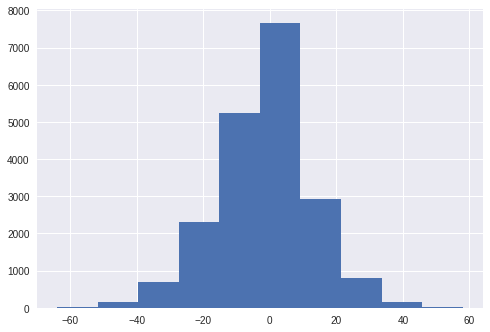
\includegraphics[width=0.7\textwidth]{graphics/lorentz_horey_distribution.png}
        \end{center}
        \caption{Distribution of Lorentz Horey values}
        \label{fig:lorentzdistribution}
    \end{small}
\end{figure}

\begin{figure}
    \begin{small}
        \begin{center}
            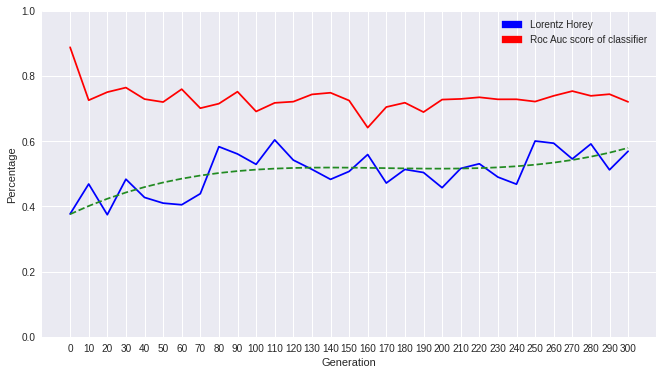
\includegraphics[width=0.95\textwidth]{graphics/lorentz_horey_trend.png}
        \end{center}
        \caption{Percentage of selected states containing the HLC Lorentz-Horey}
        \label{fig:lorentzheuristic}
    \end{small}
\end{figure}


The last heuristic we examined was the Lorentz-Horey heuristic. This heuristic is a popular heuristic in breakthrough defined in the paper by Lorentz \& Horey~\cite{lorentz:heuristic}. For this heuristic, we give each cell on the board a point value. For a given player the heuristic is then the sum of the cell values where they have pawns. The cell values can be seen in Table \ref{table:lorentzcell}. the matrix shown is flipped in the black player's point of view. The values are selected in such a way that as your pawn approach the opponent's side their value increases, having pieces on the edge isn't optimal, as such a pawn will only be able to capture in one direction and can not escape capture as easily. To select the breakpoint for Lorentz-Horey heuristic we generated 20000 states and considered the values, the resulting distribution can be seen in Figure \ref{fig:lorentzdistribution}. This distribution leads us to select the value of $5$, as a breakpoint indicating that a state has the HLC of Lorentz-Horey. The evolution of the neural network using this HLC for selection can be seen in Figure \ref{fig:lorentzheuristic}

Examining Figure~\ref{fig:lorentzheuristic}, we can see that the trend of using this HLC increases over time. As this heuristic is the one most often cited as a successful strategy in breakthrough this result is promising.

\section{Examining state properties}

To be able to view the results from the concept activation vectors it is important to know how many states we expect to have a concept so that we can know whether the model is only guessing at random or not.